%%%%%%%%%%%%%%%%%%%%%%%%%%%%%%%%%%%%%%%%%%%%%%%%%%%%%%%%%%%%%%%%%%%%%%%%%%%%%
% Баталов Семен, 2021                                                       %
%%%%%%%%%%%%%%%%%%%%%%%%%%%%%%%%%%%%%%%%%%%%%%%%%%%%%%%%%%%%%%%%%%%%%%%%%%%%%

\documentclass[12pt, a4paper]{article}
\usepackage[left=2.5cm, right=2.5cm, top=2.5cm, bottom=2.5cm]{geometry}
\usepackage[utf8]{inputenc}
\usepackage{graphicx}
\graphicspath{{./pictures/}}
\usepackage[english, russian]{babel}
\usepackage{indentfirst}
\usepackage{misccorr}
\usepackage{amsmath}

\title{Применение генетического алгоритма для решения СЛУ и ОДУ}
\author{Баталов Семен}
\date{02.03.2021}

\begin{document}
    
    \sloppy
    
    \maketitle
    
    \section{Генетический алгоритм}
    
    Генетический алгоритм~--~это эвристический алгоритм поиска, используемый 
    для решения задач оптимизации и моделирования путем случайного подбора, 
    комбинирования и вариации искомых параметров с использованием 
    механизмов, аналогичных естественному отбору в природе.
    
    Задача формализуется таким образом, чтобы её решение могло быть 
    закодировано в виде вектора (<<генотипа>>) генов, где каждый ген может 
    быть битом, числом или неким другим объектом. Можно выделить следующие 
    этапы генетического алгоритма:
    
    \begin{itemize}
        \item Инициализация
            \begin{enumerate}
                \item Задать целевую функцию (приспособленности) для особей 
                популяции
                \item Создать начальную популяцию
            \end{enumerate}
        \item Начало цикла
            \begin{enumerate}
                \item Размножение (скрещивание)
                \item Мутирование
                \item Вычислить значение целевой функции (функции 
                приспособленности) для всех особей
                \item Формирование нового поколения (селекция)
                \item Если выполняются условия остановки, то (конец цикла), 
                иначе (начало цикла)
            \end{enumerate}
    \end{itemize}
    
    Далее считаем, что каждый ген является вещественным числом. Функция 
    приспособленности зависит от задачи и будет определена позже. Условием 
    остановки считаем достижение определенного количества итераций.
    
    \section{Инструменты}
    
    Языком разработки является <<\textbf{Python}>>. Для работы с 
    генетическим алгоритмом используется библиотека 
    <<\textbf{geneticalgorithm}>>. Подробнее о программе можно узнать в 
    папке <<\textbf{source}>> проекта.
    
    \section{Решение ОДУ первого порядка}
    
    Мы рассматриваем задачу нахождения приближенного решения задачи Коши 
    обыкновенного дифференциального уравнения первого порядка (\ref{eq1}).
    
    \begin{equation}
        \dot{X} = F(t, X)
        \label{eq1}
    \end{equation}
    
    Естественно полагаем, что решение существует и единственно на промежутке 
    $(a, b) \ni t_{0}$. Не умаляя общности, рассматриваем задачу Коши 
    (\ref{eq2}). Считаем, что решение выражается через элементарные функции.
    
    \begin{equation}
        t_{0} = 0, \qquad X(t_{0}) = X_{0} = 0
        \label{eq2}
    \end{equation}
    
    Решение задачи (\ref{eq1}), (\ref{eq2}) приближаем полиномом $p$ степени 
    $deg(p) = 7$ (это число было подобрано экспериментально, с увеличением 
    степени эффективность алгоритма падает). Генами при данной постановке 
    вопроса являются коэффициенты многочлена при соответствующих степенях, 
    таким образом длина <<генотипа>> равна 7.
    
    Важно отметить, что количесво особей в каждом поколении постоянно и 
    равно 100, другие параметры алгоритма можно посмотреть в коде программы. 
    В качестве функции приспособленности используем среднее квадратичное 
    отклонение (\ref{eq3}).
    
    \begin{equation}
        Err(p) = \sqrt{\sum_{i=0}^{num - 1}\Big(\dot{p}(t_{i}) - F(t_{i}, 
            p(t_{i}))\Big)^{2} + \Big(p(t_{0})-X_{0}\Big)^{2}} 
        \label{eq3}
    \end{equation}
    
    Здесь $num$~-~количество точек в дроблении промежутка $(a, b)$. Далее 
    рассмотрим примеры решений некоторых ДУ. На рисунках слева указано 
    приближение полиномом, а справа изображено отклонение (разность 
    значений) полинома от оригинальной функции.
    
    \subsection{$\dot{X} = cos(t)$}
    
    Решение задачи Коши (\ref{eq1}), (\ref{eq2}): $X(t) = sin(t)$. 
    Промежуток задания: $(-1.5, 1.5)$. Дробление интервала осуществляется с 
    шагом 0.1.
    
    \begin{figure}[h!]
        \center
        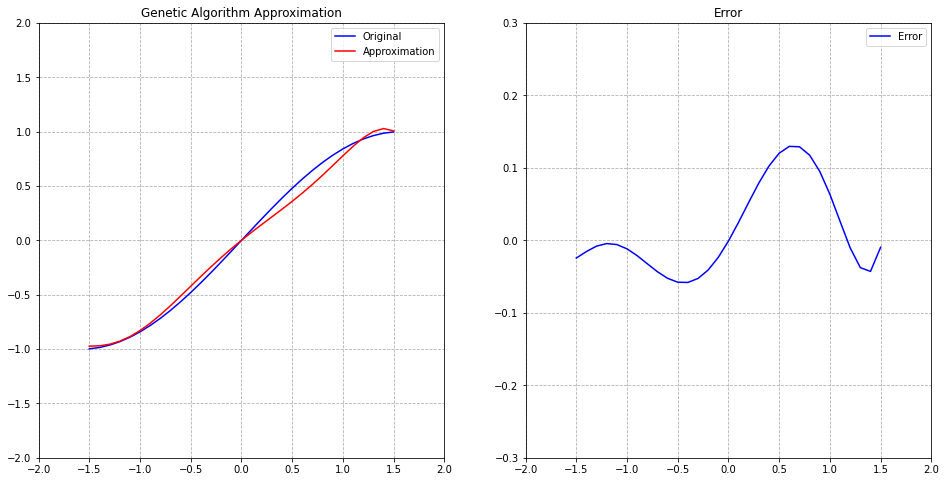
\includegraphics[width = 13cm]{f1_300.png}
        \label{image311}
        \caption{Приближенное решение $\dot{X} = cos(t)$, 300 поколений.}
    \end{figure}
    
    На рис.~\ref{image311}.1 представлен результат работы программы для 300 
    поколений. Видно, что ошибка достаточно велика. Далее представлены 
    результаты для 800 и 1000 поколений соответственно.
    
    \begin{figure}[h!]
        \center
        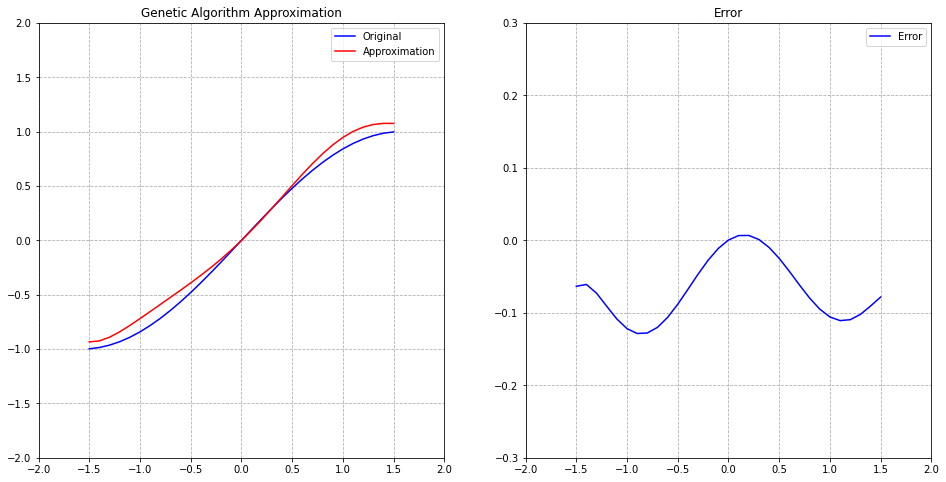
\includegraphics[width = 13cm]{f1_800.png}
        \label{image312}
        \caption{Приближенное решение $\dot{X} = cos(t)$, 800 поколений.}
    \end{figure}
    
    \begin{figure}[h!]
        \center
        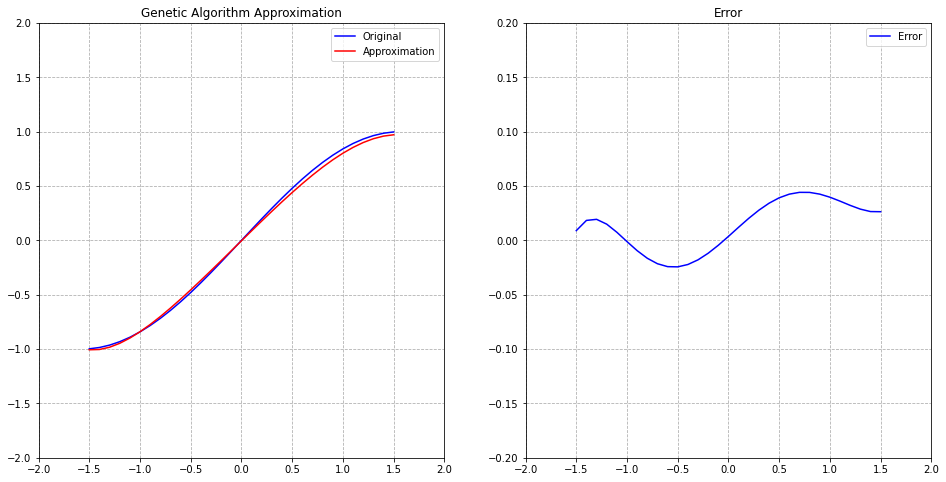
\includegraphics[width = 13cm]{f1_1000.png}
        \label{image313}
        \caption{Приближенное решение $\dot{X} = cos(t)$, 1000 поколений.}
    \end{figure}
    
    Нетрудно видеть, что на рис.~\ref{image313}.3 наименьшее отклонение 
    значений полинома от значений решения ДУ.
    
    \subsection{$\dot{X} = X^{2} + 1$}
    
    Решение задачи Коши (\ref{eq1}), (\ref{eq2}): $X(t) = tg(t)$. Промежуток 
    задания: $(-1,1)$. Дробление интервала осуществляется с шагом 0.1.
    
    В отличие от предыдущего примера, здесь зависимость точности приближения 
    от количества поколений прослеживается хуже. Лучший результат 
    представлен на рис.~\ref{image322}.2, 800 поколений.
    
    \begin{figure}[h!]
        \center
        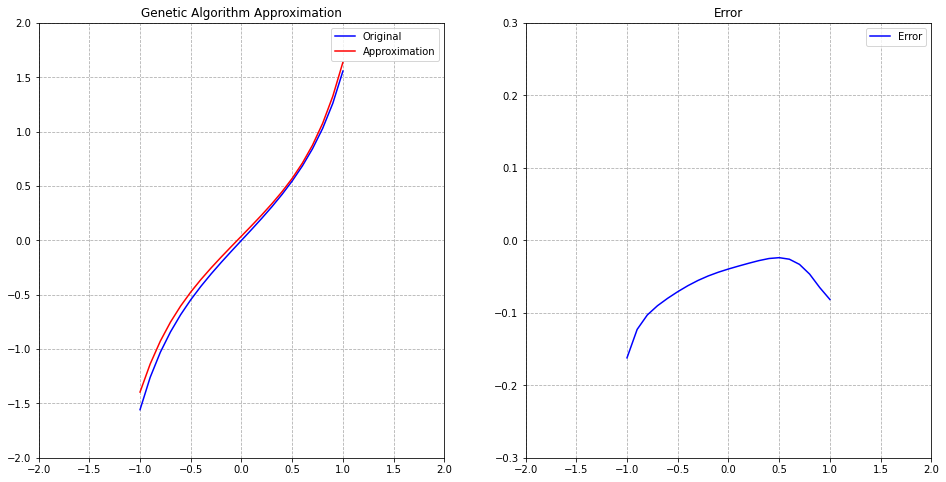
\includegraphics[width = 13cm]{f2_300.png}
        \label{image321}
        \caption{Приближенное решение $\dot{X} = X^{2} + 1$, 300 поколений.}
    \end{figure}
    
    \begin{figure}[h!]
        \center
        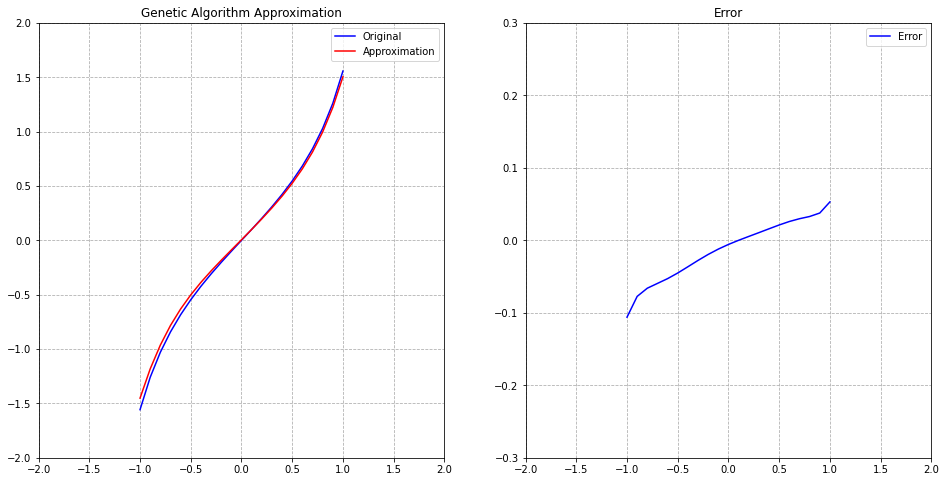
\includegraphics[width = 13cm]{f2_800.png}
        \label{image322}
        \caption{Приближенное решение $\dot{X} = X^{2} + 1$, 800 поколений.}
    \end{figure}
    
    \begin{figure}[h!]
        \center
        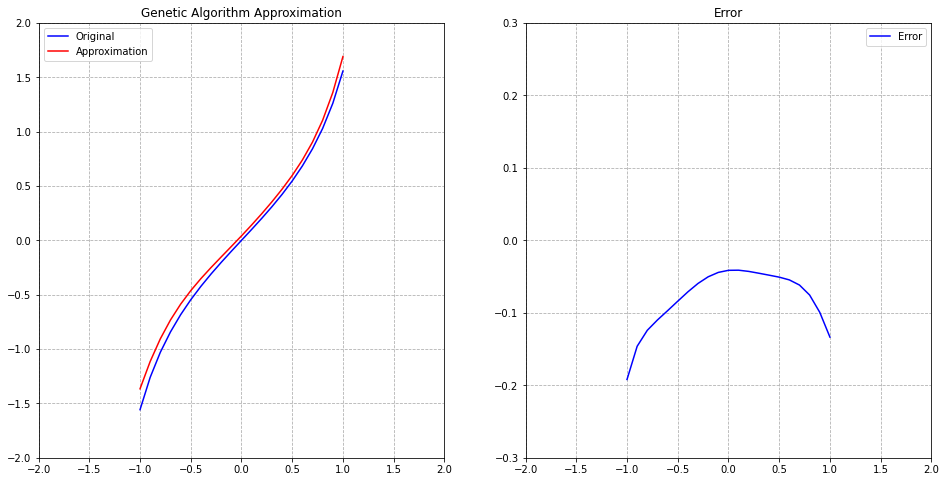
\includegraphics[width = 13cm]{f2_1000.png}
        \label{image323}
        \caption{Приближенное решение $\dot{X} = X^{2} + 1$, 1000 поколений.}
    \end{figure}
    
    \subsection{$\dot{X} = -X$}
    
    Решение задачи Коши (\ref{eq1}), (\ref{eq2}): $X(t) = -\frac{X^{2}}{2}$. 
    Промежуток задания: $(-1.5, 1.5)$. Дробление интервала осуществляется с 
    шагом 0.1.
    
    \begin{figure}[h!]
        \center
        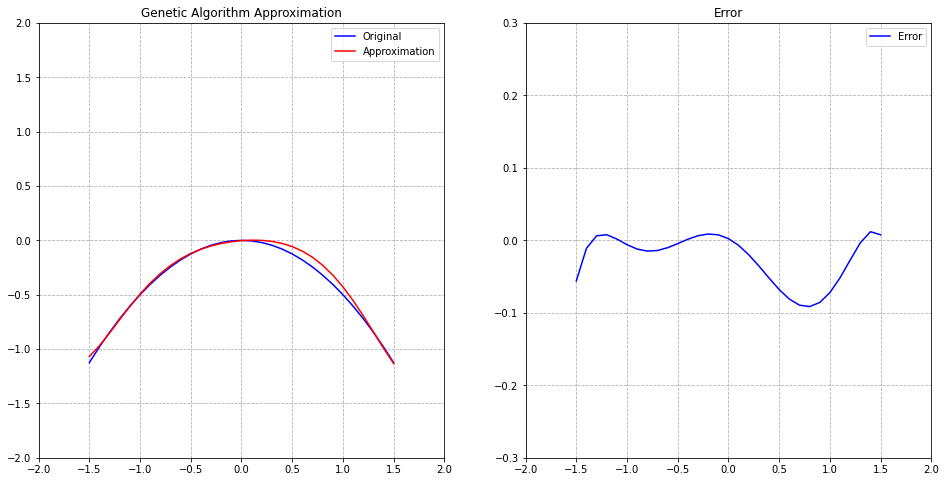
\includegraphics[width = 13cm]{f3_300.png}
        \label{image331}
        \caption{Приближенное решение $\dot{X} = -X$, 300 поколений.}
    \end{figure}
    
    До этого мы рассматривали нечетные функции, четные алгоритм тоже 
    приближает с приемлемой точностью. Стоит отметить, что результат работы 
    программы может меняться при разных запусках, это объясняется 
    вероятностной природой генетического алгоритма.
    
    \begin{figure}[h!]
        \center
        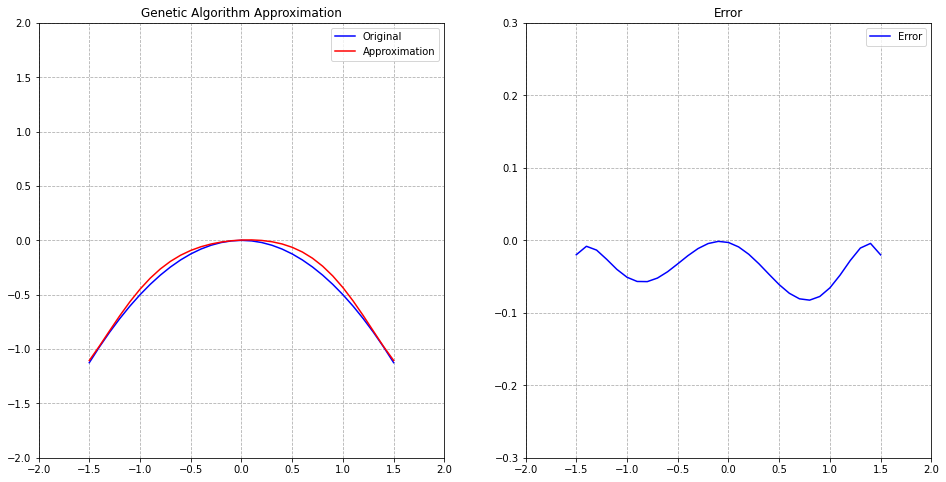
\includegraphics[width = 13cm]{f3_800.png}
        \label{image332}
        \caption{Приближенное решение $\dot{X} = -X$, 800 поколений.}
    \end{figure}
    
    Видно, что результат работы алгоритма слабо зависит от количества 
    итераций. Иногда при меньшем количестве поколений можно добиться большей 
    точности. Далее рассмотрим приближение для 1000 итераций.
    
    \begin{figure}[h!]
        \center
        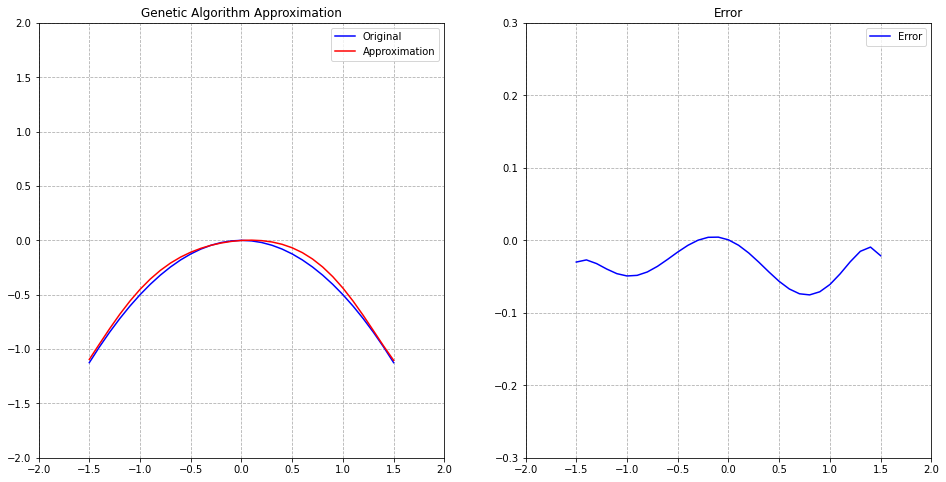
\includegraphics[width = 13cm]{f3_1000.png}
        \label{image333}
        \caption{Приближенное решение $\dot{X} = -X$, 1000 поколений.}
    \end{figure}
    
    \subsection{Выводы}
    
    В целом удалось решить проблему поиска решения задачи Коши ДУ первого 
    порядка с помощью генетического алгоритма. Однако, возникает большое 
    количество проблем, связанных с вычислением приближенного решения. Мы 
    аппроксимировали элементарные функции полиномом, это уже вносит 
    неточность в ответ, более того нельзя без потерь увеличить степень этого 
    многочлена, так как алгоритм сильно замедлится, если вообще сможет 
    сойтись. Также недостатком метода является отсутствие информации (в 
    общем случае) о диапазоне, в котором должен находится соответствующий 
    коэффициент полинома. Если диапазон задать слишком широким, то алгоритм 
    будет дольше сходиться, и точность полученного решения окажется меньшей.
    
    Таким образом, генетический алгоритм способен находить приближенное 
    решение задачи Коши ОДУ (первого порядка), выраженное полиномом, но 
    данный метод имеет много недостатков и ограничений. 
    
    \section{Решение СЛНУ}
    
    Теперь рассмотрим задачу нахождения приближенного решения системы 
    линейных неоднородных уравнений (\ref{sle1}). Будем рассматривать 
    системы трех уравнений (для систем других порядков все результаты 
    аналогичны).
    
    \begin{equation}
        \left(
        \begin{array} {ccc}
            a_{11} & a_{12} & a_{13} \\
            a_{21} & a_{22} & a_{23} \\
            a_{31} & a_{32} & a_{33} \\
        \end{array}
        \right)
        \cdot
        \left(
        \begin{array} {ccc}
            x_{1} \\
            x_{2} \\
            x_{3} \\
        \end{array}
        \right)
        =
        \left(
        \begin{array} {ccc}
            b_{1} \\
            b_{2} \\
            b_{3} \\
        \end{array}
        \right), 
        \qquad
        X_{0} =
        \left(
        \begin{array} {ccc}
            x^{0}_{1} \\
            x^{0}_{2} \\
            x^{0}_{3} \\
        \end{array}
        \right)
        \label{sle1}
    \end{equation}
    
    Будем считать, что решение системы (\ref{sle1}) существует и 
    единственно. В качестве генотипа будем брать вектор $X = (x_{1}, x_{2}, 
    x_{3})^T$. Дианазон значений для каждой координаты считаем известным 
    заранее. Важно определить функцию приспособленности. Мы будем 
    использовать сумму абсолютных значений отклонения каждой координаты 
    (\ref{sle2}).
    
    \begin{equation}
        Err(X) = \sum_{i=1}^{3} |a_{i1}x_{1} + a_{i2}x_{2} + a_{i3}x_{3} - b_{i}|
        \label{sle2}
    \end{equation}
    
    Количество итераций алгоритма будет меняться, количество особей в рамках 
    одного примера в каждом поколении постоянно. Дополнительные параметры 
    алгоритма можно увидеть в файле программы.
    
    Далее потребуется анализировать величину отклонения приближенного 
    решения системы от действительного, будем вычислять его по формуле 
    (\ref{sle3}).
    
    \begin{equation}
        Dev(X) = \sum_{i=1}^{3} |x_{i} - x^{0}_{i}|
        \label{sle3}
    \end{equation}
    
    \subsection{Пример 1}
    
    Рассмотрим СЛНУ из трех уравнений (\ref{sle4}). В соответствии с 
    решением этой системы накладываем ограничения на диапазон возможных 
    значений генов $x_{1}, x_{2}, x_{3} \in [-5, 5]$.
    
    \begin{equation}
        \left(
        \begin{array} {ccc}
            1 & 6 & 3 \\
            11 & 7 & 6 \\
            7 & 8 & 9 \\
        \end{array}
        \right)
        \cdot
        \left(
        \begin{array} {ccc}
            x_{1} \\
            x_{2} \\
            x_{3} \\
        \end{array}
        \right)
        =
        \left(
        \begin{array} {ccc}
            7 \\
            2 \\
            3 \\
        \end{array}
        \right), 
        \qquad
        X_{0} =
        \left(
        \begin{array} {ccc}
            -0.428 \\
            1.628 \\
            -0.781 \\
        \end{array}
        \right)
        \label{sle4}
    \end{equation}
    
    Запустим алгоритм для разного количества особей и числа поколений, 
    составим график зависимости отклонения (\ref{sle3}) приближенного 
    решения от действительного от числа итераций для 100 и 200 особей 
    (рис.~\ref{image411}.10). Значение ошибки в конкретном случае 
    соответствует среднему арифметическому ошибок для 10 запусков программы.
    
    \begin{figure}[h!]
        \center
        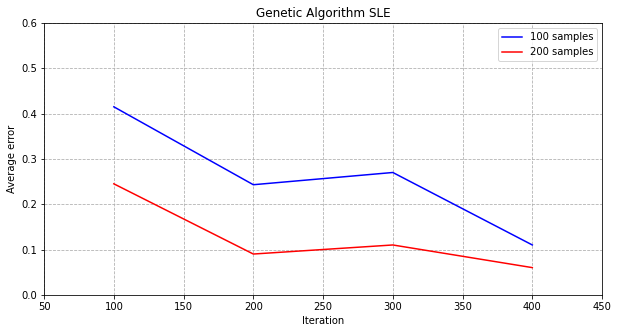
\includegraphics[width = 13cm]{sle1_3.png}
        \label{image411}
        \caption{Зависимость отклонения (\ref{sle3}) приближенного решения  
            системы (\ref{sle4}) от числа итераций генетического алгоритма.}
    \end{figure}
    
    Заметим, что на точность решения оказывют влияние оба фактора: 
    количество особей в каждом поколении, количество итераций алгоритма. При 
    меньшем количестве особей потребуется больше поколений, чтобы получить 
    требуемую точность.
    
    \subsection{Пример 2}
    
    Рассмотрим аналогичную СЛНУ из трех уравнений (\ref{sle5}). В 
    соответствии с решением этой системы накладываем ограничения на диапазон 
    возможных значений генов $x_{1}, x_{2}, x_{3} \in [-10, 10]$. Диапазон 
    значений расширился в сравнении с предыдущим примером.
    
    \begin{equation}
        \left(
        \begin{array} {ccc}
            2 & 5 & 33 \\
            10 & 11 & 61 \\
            8 & 13 & 9 \\
        \end{array}
        \right)
        \cdot
        \left(
        \begin{array} {ccc}
            x_{1} \\
            x_{2} \\
            x_{3} \\
        \end{array}
        \right)
        =
        \left(
        \begin{array} {ccc}
            16 \\
            7 \\
            32 \\
        \end{array}
        \right), 
        \qquad
        X_{0} =
        \left(
        \begin{array} {ccc}
            -5.167 \\
            5.685 \\
            -0.063 \\
        \end{array}
        \right)
        \label{sle5}
    \end{equation}
    
    Запустим алгоритм для разного количества особей и числа поколений, 
    составим график зависимости отклонения (\ref{sle3}) приближенного 
    решения от действительного от числа итераций для 100 и 200 особей 
    (рис.~\ref{image421}.11). Значение ошибки в конкретном случае 
    соответствует среднему арифметическому ошибок для 10 запусков программы.
    
    \begin{figure}[h!]
        \center
        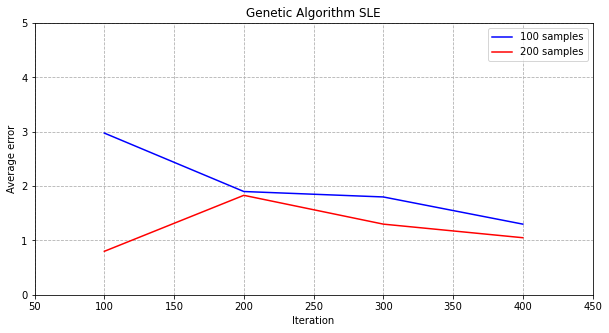
\includegraphics[width = 13cm]{sle2_3.png}
        \label{image421}
        \caption{Зависимость отклонения (\ref{sle3}) приближенного решения  
            системы (\ref{sle5}) от числа итераций генетического алгоритма.}
    \end{figure}
    
    В целом результаты аналогичны результатам примера 1. Ярко выражена 
    зависимость точности решения от числа особей в каждом поколении. Число 
    итераций алгоритма также влияет на точность результата.
    
    \subsection{Вывод}
    
    При решении СЛНУ при помощи генетического алгоритма существенное влияние 
    на точность решения оказывают число итераций (поколений) алгоритма и 
    количество особей в каждом поколении. В соответствии с выбранной 
    метрикой (\ref{sle2}), (\ref{sle3}) и постановкой вопроса можно 
    заключить, что алгоритм находит решение задачи с достаточной точностью. 
    
    \section{Общий вывод}
    
    В результате проведенной работы во многом стали очевидны положительные и 
    отрицательные стороны применения генетического алгоритма. Стоит отметить 
    его простоту, не требуется понимать всю специфику задачи, достаточно 
    правильно подобрать метрику, составить генотип и установить 
    вспомогательные параметры, чтобы получить достаточно точное решение. 
    Однако есть серьезный недостаток, связанный с вероятностной природой 
    алгоритма. Нельзя абсолютно точно предсказать исход его работы (во 
    многих экспериментах он работал нестабильно). Подобный недостаток сужает 
    круг задач, в которых генетический алгоритм может быть применен.
    
\end{document}